\documentclass[letterpaper]{article}
\usepackage[square,sort,comma,numbers]{natbib}
\usepackage{array}
%====================================================================%
../../../../tex/scufftex.tex
\graphicspath{{figures/}}
\renewcommand{\wt}{\widetilde}

%------------------------------------------------------------
%------------------------------------------------------------
%- Special commands for this document -----------------------
%------------------------------------------------------------
%------------------------------------------------------------

%------------------------------------------------------------
%------------------------------------------------------------
%- Document header  -----------------------------------------
%------------------------------------------------------------
%------------------------------------------------------------
\title {Implicit handling of multilayered dielectric substrates 
        in {\sc scuff-static}
       }
\author {Homer Reid}
\date {March 25, 2017}

%------------------------------------------------------------
%------------------------------------------------------------
%- Start of actual document
%------------------------------------------------------------
%------------------------------------------------------------

\begin{document}
\pagestyle{myheadings}
\markright{Homer Reid: Electrostatic GF above PCB} 
\maketitle

\tableofcontents

%====================================================================%
%====================================================================%
%====================================================================%
\newpage
%####################################################################%
\begin{figure}
\begin{center}
\resizebox{\textwidth}{!}{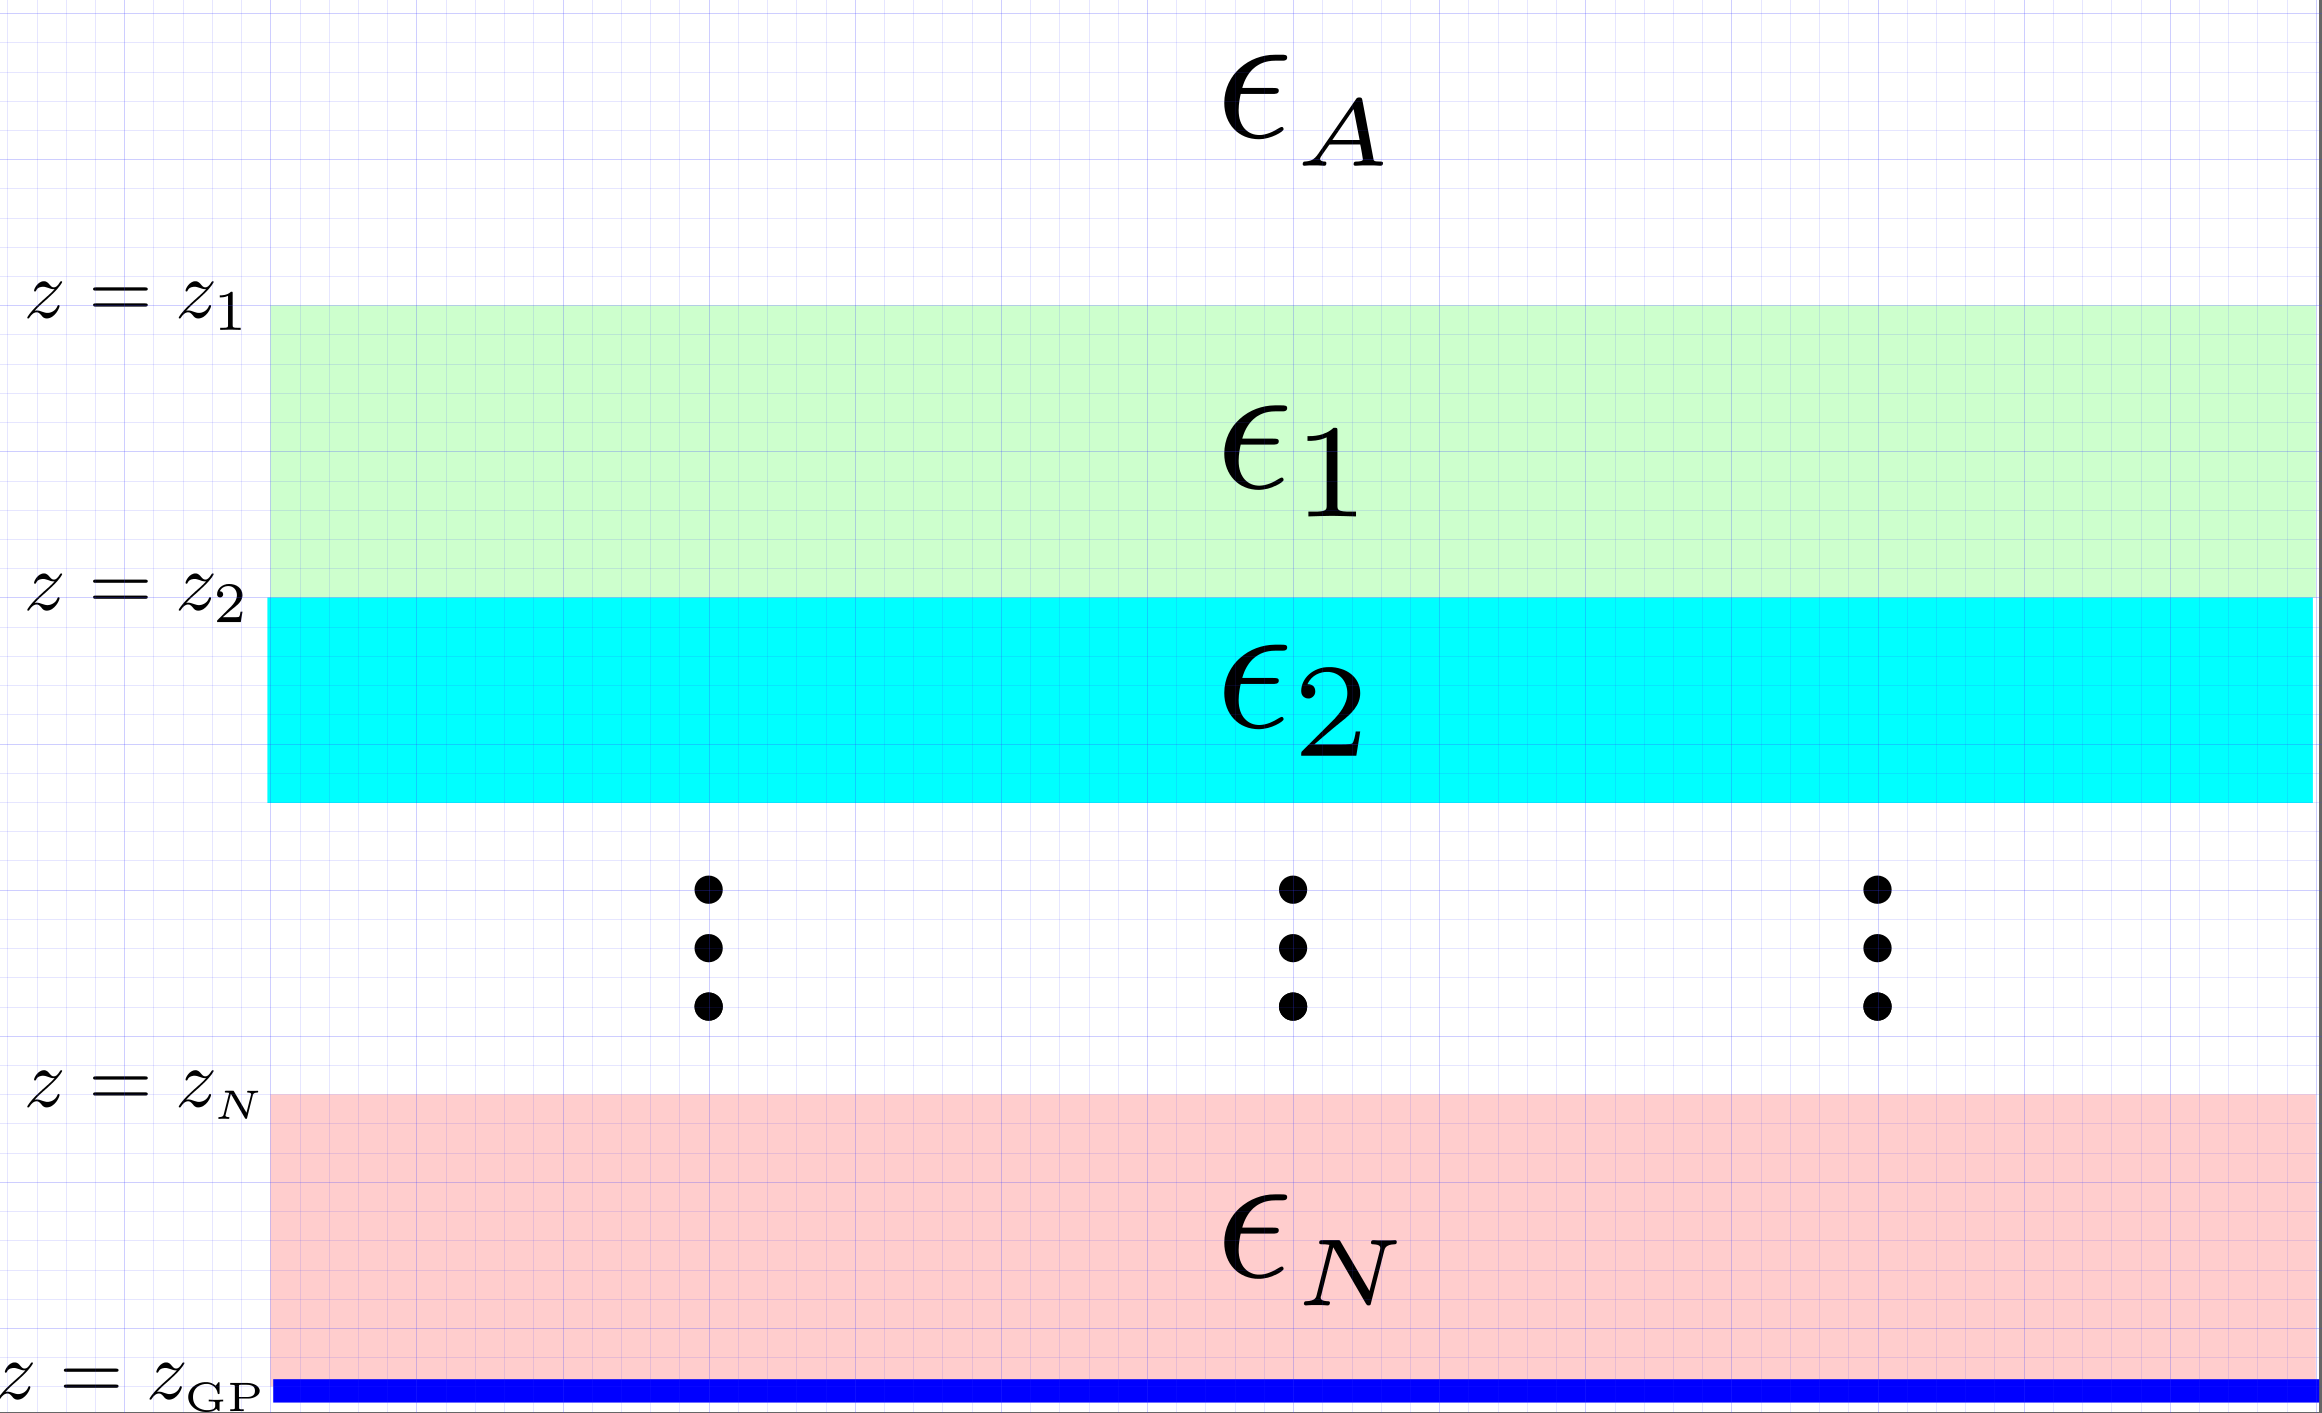
\includegraphics{DielectricSubstrateCartoon.pdf}}
\caption{Geometry of the layered dielectric substrate. The $n$th layer
has relative DC permittivity $\epsilon_n$, and its upper surface
lies at $z=z_n$. The ground plane, if present, lies
at $z=z\subt{GP}.$}
\label{SubstrateGeometryFigure}
\end{center}
\end{figure}
%####################################################################%
\section{Overview}

In this memo I describe an extension to the {\sc scuff-em}
electrostatics module to allow implicit treatment of
layered substrates consisting of multiple dielectric layers,
of arbitrary thicknesses and permittivities, with an optional
perfectly conducting ground plane (Figure 1). (The subscripts ``D'' and
``S'' stand for ``destination'' and ``source.'')\footnote{Note 
that, if there is no ground plane, then the bottommost 
layer in Figure \ref{SubstrateGeometryFigure})
(layer $N$) is assumed
to be infinitely thick (it has no lower surface). Thus, a physical 
substrate consisting of $M$ finite-thickness dielectric layers with 
no ground plane is treated here as a stack of $N=M+1$ layers in which
the bottommost layer is vacuum, i.e. $\epsilon\subt{$N$}=1.$}

In Section \ref{TheorySection} I construct an expression for the potential
at $\vb x\subt{D}=(x\subt{D},y\subt{D},z\subt{D})$
due to a unit-strength point charge at
$\vb x\subt{S}=(x\subt{S},y\subt{S},z\subt{S})$ in the presence
of the multilayered substrate (Figure 1).

In Section \ref{ImplementationSection} I document the usage
of this new feature in {\sc scuff-static} calculations.

%====================================================================%
%====================================================================%
%====================================================================%
\newpage
\section{Theory}
\label{TheorySection}
%####################################################################%
\begin{figure}
\begin{center}
\resizebox{\textwidth}{!}{\includegraphics{DielectricSubstrateSigmaLayers.pdf}}
\caption{In the surface-integral-equation picture of the geometry of Figure
         \ref{SubstrateGeometryFigure}, the effect of the dielectric substrate
         is represented by a collection of surface-charge layers
         $\{\sigma_{n}(\vbrho)\}$, where $\sigma_n$ lives at the 
         upper surface of dielectric layer $n$, i.e. at $z=z_n$.}
\label{SigmaLayersFigure}
\end{center}
\end{figure}
%####################################################################%
In keeping with the spirit of the surface-integral-equation method, I
will proceed by determining the effective surface-charge densities
induced at each dielectric interface by the point source
(Figure \ref{SigmaLayersFigure}). For an $N$-layer substrate
there are $N$ such layers, with the surface-charge density at
the interface between layers $n-1$ and $n$ denoted by $\sigma_n(\vbrho)$.
Note that I do not include a
surface-charge layer for the ground plane, whose effect I capture
implicitly via the method of images. 

\subsection{Expressing $G$ in terms of $\sigma$}

I write the full Green's function $G(\vb x\subt{D}, \vb x\subt{S})$---the 
potential at $\vb x\subt{D}=(\vbrho\subt{D},z\subt{D})$ 
due to a unit-strength point charge
at $\vb x\subt{S}=(\vbrho\subt{S},z\subt{S})$---as a sum
of contributions from 
 \textbf{(a)} the point source itself, 
 \textbf{(b)} the image charge of the point source (if a ground plane is
 present),
and 
 \textbf{(c)} the surface-charge layers:
%====================================================================%
\begin{align*}
 G(\vb x\subt{D}, \vb x\subt{S}) 
&=                G_0(\vb x\subt{D}, \vb x\subt{S}) 
 + \delta\subt{GP}G_0(\vb x\subt{D}, \vb x\subt{S}^*)
 + \sum_n \phi(\vb x\subt{D}; \sigma_n, z_n)
%--------------------------------------------------------------------%
\intertext{where}
%--------------------------------------------------------------------%
  G_0(\vb x\subt{D}, \vb x\subt{S})
&= \frac{1}{4\pi|\vb x\subt{D}-\vb x\subt{S}|}
%--------------------------------------------------------------------%
\intertext{is the bare vacuum Green's function,}
%--------------------------------------------------------------------%
\vb x\subt{S}^* 
&= (x\subt{S}, y\subt{S}, z\subt{S}^*),
  \quad z\subt{S}^* \equiv 2z\subt{GP}-z\subt{S} 
\intertext{are the coordinates of the image charge due to the 
ground plane at $z=z\subt{GP}$,}
%--------------------------------------------------------------------%
\delta\subt{GP}&=
 \begin{cases} 0, \qquad &\text{no ground plane} \\
               1, \qquad &\text{ground plane}
 \end{cases}
\end{align*}
%====================================================================%
and $\phi(\vb x; \sigma, z)$ is the potential at $\vb x$ due
to a surface-charge layer $\sigma(\vbrho)$ at $z$.
Putting
$\vbrho\equiv (\vbrho\subt{D}-\vbrho\subt{S})$
and $\rho\equiv |\vbrho|$ and using the results of
Appendix \ref{SurfaceChargeLayerAppendix}, we have
%====================================================================%
\begin{align*}
 \mc G(\rho; z\subt{D}, z\subt{S})
&=   G_0(\rho; z\subt{D}, z\subt{S})
  +\delta\subt{GP} G_0(\rho; z\subt{D}, z\subt{S}^*)
  + \sum_n \int \frac{dq}{4\pi} \wt{\sigma}_n(q) J_0(q\rho)
    \zeta(z\subt{D},z_n)
\intertext{and the $z$-directed electric field $E_z=-\pard{G}{z}$ reads}
E_z(\rho; z\subt{D}, z\subt{S})
&=  E_{z0}(\rho; z\subt{D}, z\subt{S})
  +\delta\subt{GP} E_{z0}(\rho; z\subt{D}, z\subt{S}^*)
  + \sum_n \int \frac{qdq}{4\pi} \wt{\sigma}_n(q) J_0(q\rho)
    \xi(z\subt{D},z_n)
\end{align*}
%====================================================================%
with 
%====================================================================%
$$ E_{z0}(\rho, z, z^\prime)
   \equiv 
   \frac{1}{4\pi[\rho^2 + (z-z^\prime)^2]^{3/2}}.
$$
%====================================================================%
The functions $\zeta$ and $\xi$ are defined in 
Appendix \ref{SurfaceChargeLayerAppendix}.

%=================================================
%=================================================
%=================================================
\subsection{Applying boundary conditions}

The boundary condition at the interface between dielectric
layers $m-1$ and $m$ reads
%====================================================================%
$$ \epsilon_{m-1} 
   E_{z}\Big(\rho; z_m^+; z\subt{S}\Big)
 = \epsilon_{m} 
   E_{z}\Big(\rho; z_m^-; z\subt{S}\Big)
$$
%====================================================================%
with the convention $\epsilon_0=1$. Using the above results, we have
%====================================================================%
\begin{align*}
&\int \frac{qdq}{4\pi} J_0(q\rho)
   \sum_{n}
   \Big[ \epsilon_{m-1} \xi(q; z_m^+; z_n)
        -\epsilon_{m  } \xi(q; z_m^-; z_n)
   \Big]\wt{\sigma}_n(q)
\\
&\qquad
  =-\big( \epsilon_{m-1} - \epsilon_m\big)
    \Big[                  E_{z0}(\rho; z_m; z\subt{S}) 
          - \delta\subt{GP}E_{z0}(\rho; z_m, z\subt{S}^*)
    \Big]
\end{align*}
%====================================================================%
or, inverse Bessel-transforming\footnote{Multiply both 
sides by $\rho J_0(q^\prime\rho)$, integrate over all $\rho$, and
use 
$$\int_0^\infty \rho J_0(q\rho) J_0(q^\prime \rho) d\rho = 
  \frac{1}{q}\delta(q-q^\prime).
$$} and rearranging slightly,
%====================================================================%
\numeq{MSigmae}
{
\sum_n
 \underbrace{
 \left[
 \frac{ \epsilon_{m-1} \xi(q; z_m^+; z_n)
        -\epsilon_{m  } \xi(q; z_m^-; z_n)
      }{ \epsilon_{m-1}-\epsilon_m}
 \right]}_{M_{mn}} \wt{\sigma}_n(q)
=-\underbrace{4\pi\Big[ 
                  \wt{E_{z0}}(q, z_m, z\subt{S}) 
              - \delta\subt{GP}\wt{E_{z0}}(q, z_m, z\subt{S}^*)
                 \Big]
            }_{e_m}
}
%====================================================================%
with
%====================================================================%
\begin{align*}
 4\pi \wt{E_{z0}}(q,z,z^\prime)
&=4\pi \int_0^\infty \rho J_0(q\rho) E_{z0}(\rho,z,z^\prime)\,d\rho
\\
&=e^{-q|z-z^\prime|}.
\end{align*}
%====================================================================%
Equation (\ref{MSigmae}) is an $N\times N$ linear system of the form
%====================================================================%
$$ \vb M \wt{\vbsigma} = \vb e$$
%====================================================================%
that we may solve to compute the Fourier transforms
$\wt{\sigma_n}(q)$
of the surface-charge densities at each dielectric interface.
The elements of the $\vb M$ matrix and $\vb e$ vector read
%====================================================================%
\begin{align*}
 M_{mn}
&= \begin{dcases}
    \xi(q; z_m; z_n), \qquad &m\ne n 
    \\
    \frac{  \epsilon_{m-1} \xi(q; z_m^+; z_m)
           -\epsilon_{m  } \xi(q; z_m^-; z_m)
         }{ \epsilon_{m-1}-\epsilon_m}, \qquad &m=n \\
  \end{dcases}
\\
e_m&=-e^{-q|z_m-z\subt{S}|} + \delta\subt{GP}e^{-q|z_m-z\subt{S}^*|}.
\end{align*}
%====================================================================%

%====================================================================%
%====================================================================%
%====================================================================%
\newpage
\section{Implementation in {\sc scuff-em}}
\label{ImplementationSection}

\subsection{Substrate definition file}

Referring to Figure (\ref{SubstrateGeometryFigure}),
a substrate geometry is specified by
\begin{itemize}
 \item the $z$-coordinate of the upper surface of each dielectric layer
 \item the permittivity of each layer
 \item the $z$-coordinate of the optional ground plane.
\end{itemize}

This data is specified to {\sc scuff-em} in the
form of a simple text file (conventionally given file
extension \texttt{.substrate}) consisting of one line for each
dielelectric layer plus an optional line specifying the ground 
plane, of the form

\medskip

%====================================================================%
\begin{verbcode}
z1  Material1
z2  Material2
...
zN  MaterialN
zGP GROUNDPLANE
\end{verbcode}
%====================================================================%

\medskip

where e.g.
%====================================================================%
\begin{itemize}
 \item \texttt{z1} is the $z$-coordinate of the upper surface of
       layer 1
 \item \texttt{Material1} is a {\sc scuff-em} material designation
       describing the material of layer 1
 \item The optional 
       final line, which invokes the fixed keyword \texttt{GROUNDPLANE},
       specifies that a perfectly-conducting ground plane lives at 
       coordinate $z=\texttt{zGP}$.
\end{itemize}
%====================================================================%

Here are some examples of \texttt{.substrate} files:

\begin{itemize}

\item An infinite-thickness dielectric slab with $\epsilon_r=4$ filling
the lower half-space:

\medskip
%====================================================================%
\begin{verbcode}
0 CONST_EPS_4
\end{verbcode}
%====================================================================%
\medskip

\item A finite-thickness dielectric slab with $\epsilon_r=4$
and thickness 1 whose upper surface is the $xy$ plane:

%====================================================================%
\medskip
\begin{verbcode}
 0 CONST_EPS_4
-1 VACUUM
\end{verbcode}
%====================================================================%

\item The same finite-thickness slab as before, but now 
lying atop a ground plane:

%====================================================================%
\medskip
\begin{verbcode}
 0 CONST_EPS_4
-1 GROUNDPLANE
\end{verbcode}
%====================================================================%
\end{itemize}

%====================================================================%
%====================================================================%
%====================================================================%
\appendix
\newpage
\section{Potential due to surface-charge layer}
\label{SurfaceChargeLayerAppendix}

In this appendix I derive an expression for the potential due
to a 2D layer of surface charge $\sigma(x,y)$
parallel to the $xy$ plane and lying a fixed distance above 
or below that plane.

%=================================================
%=================================================
%=================================================
\subsubsection*{2D Fourier representation of free-space Green's function}

The 3D Fourier representation of the free-space Green's function---the
potential at $\vb x\subt{D}=(\vbrho\subt{D},z\subt{D})$ due to a point charge at 
$\vb x\subt{S}=(\vbrho\subt{S},z\subt{S})$ (where the ``D'' and ``S'' 
subscripts label the ``destination'' and ``source'' points respectively)---is
%====================================================================%
\begin{align}
G_0(\vb x\subt{D}, \vb x\subt{S})
&=
 \frac{1}{4\pi |\vb x\subt{D}-\vb x\subt{S}|}
\nn
 &=\int \frac{d^3 \vb k}{(2\pi)^3}
        \frac{e^{i\vb k \cdot (\vb x-\vb x^\prime)}}{|\vb k|^2}
\nonumber
\intertext{Evaluating the $k_z$ integral yields the 2D Fourier representation:}
 &=\frac{1}{2}\int \frac{d^2 \vb q}{(2\pi)^2}
        \frac{e^{i\vb q\cdot (\vbrho\subt{D} - \vbrho\subt{S})-q|z\subt{D}-z\subt{S}|}}{q},
 \qquad  \vb   q\equiv  \vb k_\parallel,
 \quad        q\equiv |\vb q|.
\label{G02D}
\end{align}
%====================================================================%

%=================================================
%=================================================
%=================================================
\subsubsection*{Potential due to surface-charge layer at $z=z\subt{S}$}

Using (\ref{G02D}), 
the potential at $\vb x\subt{D}=(\vbrho\subt{D},z\subt{D})$
due to a surface-charge layer $\sigma(\vbrho\subt{S})$ at
$z=z\subt{S}$ is
%====================================================================%
\begin{align}
 \phi(\vbrho\subt{D}, z\subt{D})
   &=\int \, G_0(\vbrho\subt{D}, z\subt{D}; \vbrho\subt{S}, z\subt{S})
     \sigma(\vbrho\subt{S}) \,d \vbrho\subt{S}
\nn
   &=\frac{1}{2} \int \frac{d \vb q}{(2\pi)^2}
     \frac{e^{i\vb q \cdot \vbrho\subt{D} - q|z\subt{D}-z\subt{S}|}}{q}
     \underbrace{\int d\vbrho\subt{S} \, \sigma(\vbrho\subt{S}) \, e^{-i\vb q \cdot \vbrho\subt{S}}}
               _{\wt{\sigma}(\vb q)}
\nn
   &=\int \frac{d \vb q}{(2\pi)^2}
     \frac{\wt\sigma(\vb q)e^{i\vb q \cdot \vbrho\subt{D} - q|z\subt{D}-z\subt{S}|}}{2q}
\label{GSurface}
\end{align}
%====================================================================%
where $\wt \sigma$ is the Fourier transform of $\sigma$.
For circularly-symmetric cases in which $\wt \sigma$ depends only
on the magnitude of $\vb q$, as will be the case here,
this can be simplified to read
%====================================================================%
\numeq{PhiSurfaceLayer}
{
\phi(\vbrho\subt{D}, z\subt{D})
   =\int \frac{dq}{4\pi} \wt \sigma(q) J_0(q\rho\subt{D}) e^{-q|z\subt{D}-z\subt{S}|}
}
%====================================================================%
with $\rho\subt{D}=|\vbrho\subt{D}|$.

%=================================================
%=================================================
%=================================================
\subsubsection*{Potential due to surface-charge layer in presence of 
                ground plane}

In the presence of an infinitely conducting
ground plane at $z=z\subt{GP} < z\subt{S}$, the contribution of 
each infinitesimal surface-charge element at $z=z\subt{S}$ is
augmented by an image-charge element of the opposite sign at
$z=z\subt{GP}-\overline{z\subt{S}}$, where I defined
$\overline{z\subt{S}}\equiv z\subt{S}-z\subt{GP}.$
The form of the potential due to the surface-charge layer plus ground plane
now depends on whether the evaluation point lies above or below 
the surface-charge layer:
%====================================================================%
\begin{align}
\phi(\vbrho\subt{D},z\subt{D})
 &=\int \frac{dq}{2\pi} \wt \sigma(q) J_0(q\rho\subt{D})
 \begin{dcases} 
     e^{-q\overline{z\subt{D}}}\sinh q \overline{z\subt{S}},
    \qquad &z\subt{D} > z\subt{S}
    \\
     e^{-q\overline{z\subt{S}}}\sinh q \overline{z\subt{D}},
    \qquad z\subt{GP} < &z\subt{D} < z\subt{S}
 \end{dcases}
\label{PhiSurfaceLayerGP}
\end{align}
%====================================================================%
where $\overline{z\subt{D}}\equiv z\subt{D}-z\subt{GP}.$
I will write (\ref{PhiSurfaceLayer}) and (\ref{PhiSurfaceLayerGP})
in the common form
%====================================================================%
\numeq{PhiSigmaCommonForm}
{
\phi(\vbrho\subt{D},z\subt{D}) = 
 \int \frac{dq}{4\pi} \wt \sigma(q) J_0(q\rho\subt{D}) \zeta(q; z\subt{D}; z\subt{S})
}
%====================================================================%
where 
%====================================================================%
$$
 \zeta(q; z\subt{D}; z\subt{S})
 \equiv
 \begin{dcases}
  \zeta\subt{NGP}(q; z\subt{D}; z\subt{S})
  \equiv e^{-q|z\subt{D}-z\subt{S}|},
  \qquad &\text{no ground plane} 
  \\[10pt]
  \zeta\subt{GP}(q; z\subt{D}; z\subt{S}),
  \equiv 2 e^{-q\overline{z\subt{$>$}}} \sinh q\overline{z\subt{$<$}}
  \qquad &\text{ground plane}
 \end{dcases}
$$
with $\overline{z}\equiv z-z\subt{GP}$
and $z\subt{$>$}$ ($z\subt{$<$}$)
the greater (lesser) of $z\subt{D},z\subt{S}$.

I will also define a function $\xi$ according to
%====================================================================%
$$ \frac{d}{dz\subt{D}} \zeta(q; z\subt{D}; z\subt{S})
   \equiv -q\xi(q; z\subt{D}; z\subt{S}).
$$
%====================================================================%
Then one finds
%====================================================================%
\begin{align*}
  \xi\subt{NGP}(q; z\subt{D}; z\subt{S})
 &\equiv \text{sgn}(z\subt{D}-z\subt{S})e^{-q|z\subt{D}-z\subt{S}|}
\\
  \xi\subt{GP}(q; z\subt{D}; z\subt{S})
 &\equiv 
   \begin{dcases}
     +2 e^{-q\overline{z\subt{D}}} \sinh q\overline{z\subt{S}},
      \\
     -2 e^{-q\overline{z\subt{S}}} \cosh q\overline{z\subt{D}},
      \qquad &z\subt{D}<z\subt{S} 
   \end{dcases}
\end{align*}
%====================================================================%

%=================================================
%=================================================
%=================================================
\subsubsection*{$\vb E$-field components}
Taking derivatives of (\ref{PhiSigmaCommonForm}) yields
\begin{align*}
 E_x &= -\pard{\phi}{x}
 = \frac{x\subt{D}}{\rho\subt{D}}
    \int \frac{qdq}{2\pi} \wt{\sigma}(q) J_1(q\rho\subt{D})
         \zeta(q; z\subt{D}; z\subt{S})
\\
 E_y &= -\pard{\phi}{y}
 = \frac{y\subt{D}}{\rho\subt{D}}
    \int \frac{qdq}{2\pi} \wt{\sigma}(q) J_1(q\rho\subt{D})
         \zeta(q; z\subt{D}; z\subt{S})
\\
 E_z &= -\pard{\phi}{z}
 =  \int \frac{qdq}{2\pi} \wt{\sigma}(q) J_0(q\rho\subt{D})
         \xi(q; z\subt{D}; z\subt{S}).
\end{align*}

\end{document}
